\begin{frame}
\begin{itemize}
    \item \textbf{\color{red}{What are Normalizing Flows}}
    \item NICE
    \item RealNVP
    \item GLOW
    \item GamePlan
    \item Results
\end{itemize}
\end{frame}

\begin{frame}
    \frametitle{What are Normalizing Flows? (Steven)}
    \begin{itemize}
        \item Generative models, like GANs and VAEs.  \footnote{Source:
    https://lilianweng.github.io/lil-log/2018/10/13/flow-based-deep-generative-models.html}
        \item Gets \textbf{explicit} representation of density function (GANs
            and VAEs get implicit).
        \item Sequence of invertible transformations (e.g. $f(x) = \sigma x +
            \mu$ and $f^{-1}(x) = \sigma x - \mu$)
    \end{itemize}
    \center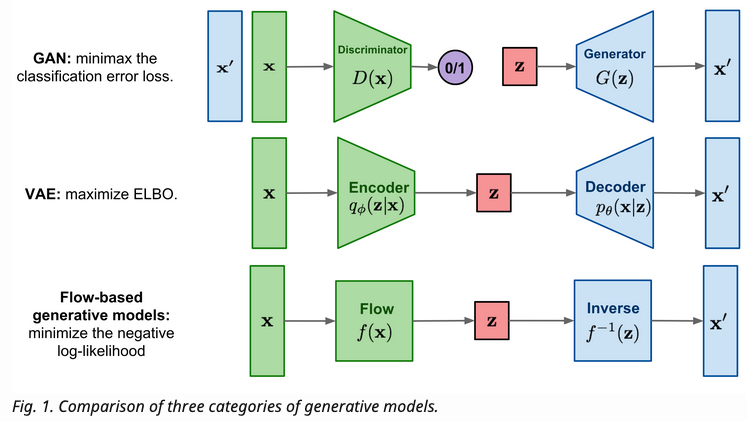
\includegraphics[width=0.75\textwidth]{GenerativeModels.png}
\end{frame}

\begin{frame}
    \frametitle{What are Normalizing Flows? (Steven)}
    \center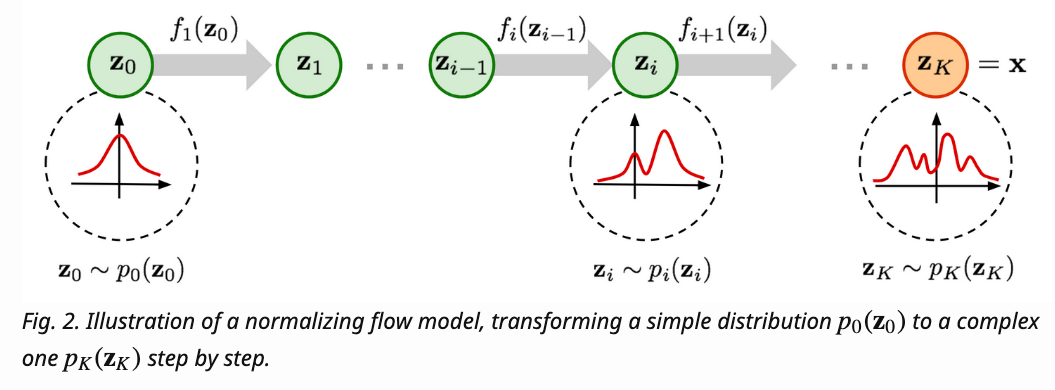
\includegraphics[width=0.95\textwidth]{NFs.png}
\end{frame}

\begin{frame}
    \frametitle{What are Normalizing Flows? (Steven)}
    \begin{itemize}
        \item Can get sharp images with log-liklihood (goodness of fit).
        \item Can explore latent space and generate different modes (e.g. We can
            turn a person old if we know where old people are in the
            distribution)
        \item Need determinant of Jacobian (use LU Decomposition to make
            faster)
        \item Need \textbf{lots} of data for high dimensional problems.
    \end{itemize}
\end{frame}

